\documentclass{standalone}

\usepackage{tikz}

\begin{document}
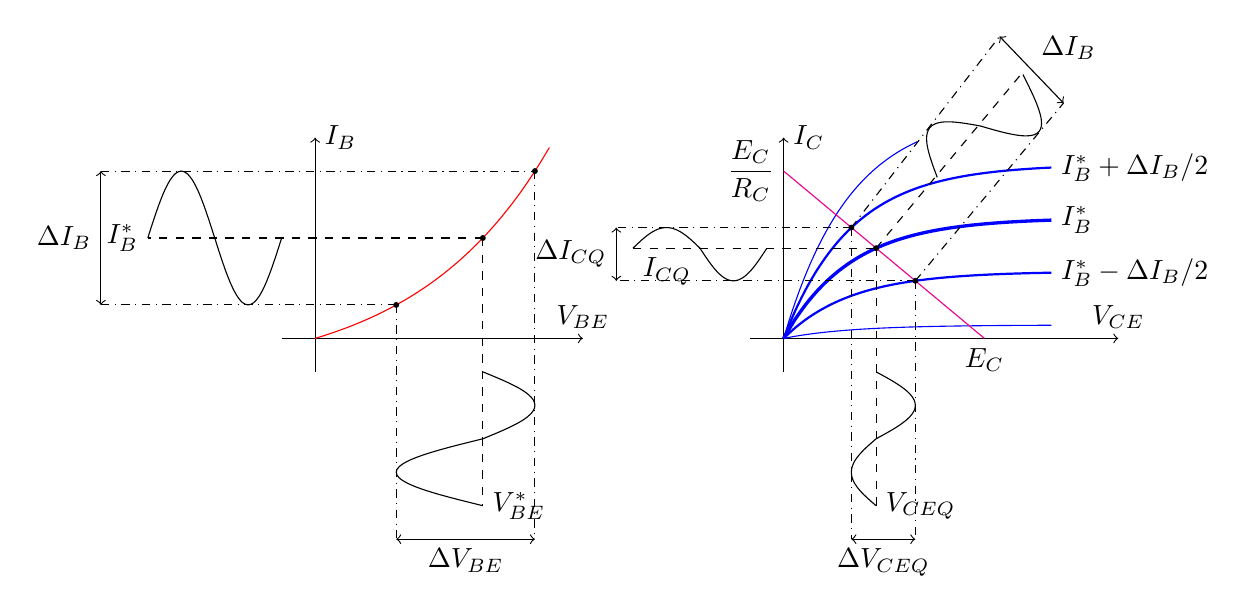
\begin{tikzpicture}[scale=1.7]
    \draw[->](-0.25,0)--(2,0)node[above]{$V_{BE}$};
    \draw[->](0,-0.25)--(0,1.5)node[right]{$I_B$};

    \draw[red,smooth, domain=0:1.75]plot (\x, {0.3*(e^((\x))-1)});

    \filldraw[black](1.2528,0.75)circle(0.5pt);
    \draw[dashed](1.2528,0.75)--(-1.25,0.75)node[left]{$I_B^*$};

    \draw[smooth, domain=-1.25:-0.25]plot(\x,{0.5*sin(2*pi*(\x+1.25) r)+0.75});
    \draw[dashdotted](-1.6,0.25)--(0.606,0.25);
    \draw[dashdotted](-1.6,1.25)--(1.642,1.25);
    \draw[<->](-1.6,0.25)--(-1.6,1.25)node[midway, left]{$\Delta I_B$};
    \filldraw[black](0.606,0.25)circle(0.5pt);
    \filldraw[black](1.642,1.25)circle(0.5pt);

    \draw[rotate=-90,smooth,domain=0.25:0.75]plot(\x,{0.389*sin(2*pi*(\x-0.25) r)+1.253});
    \draw[rotate=-90,smooth,domain=0.75:1.25]plot(\x,{0.647*sin(2*pi*(\x-0.25) r)+1.253});

    \draw[dashdotted](0.606,0.25)--(0.606,-1.5);
    \draw[dashdotted](1.642,1.25)--(1.642,-1.5);
    \draw[dashed](1.2528,0.75)--(1.2528,-1.25)node[right]{$V_{BE}^*$};
    \draw[<->](1.642,-1.5)--(0.606,-1.5)node[midway, below]{$\Delta V_{BE}$};


    \draw[->](3.25,0)--(6,0)node[above]{$V_{CE}$};
    \draw[->](3.5,-0.25)--(3.5,1.5)node[right]{$I_C$};

    \draw[blue, smooth, domain=3.5:5.5]plot (\x,{0.1*(1-e^(-2*(\x-3.5)))});
    \draw[thick,blue, smooth, domain=3.5:5.5]plot (\x,{0.5*(1-e^(-2*(\x-3.5)))});
    \draw[very thick,blue, smooth, domain=3.5:5.5]plot (\x,{0.9*(1-e^(-2*(\x-3.5)))});
    \draw[thick,blue, smooth, domain=3.5:5.5]plot (\x,{1.3*(1-e^(-2*(\x-3.5)))});
    \draw[blue, smooth, domain=3.5:4.5]plot (\x,{1.7*(1-e^(-2*(\x-3.5)))});
    \draw[magenta](3.5,1.25)node[left,black]{$\displaystyle\frac{E_C}{R_C}$}--(5,0)node[below,black]{$E_C$};
    \node[right]at(5.5,0.884){$I_B^*$};
    \node[right]at(5.5,1.276){$I_B^*+\Delta I_B/2$};
    \node[right]at(5.5,0.491){$I_B^*-\Delta I_B/2$};


    \filldraw[black](4.191,0.674)circle(0.5pt);    
    \filldraw[black](4.006,0.828)circle(0.5pt);
    \filldraw[black](4.484,0.43)circle(0.5pt);

    \draw[dashdotted](4.006,0.828)--(2.25,0.828);
    \draw[dashdotted](4.484,0.43)--(2.25,0.43);
    \draw[<->](2.25,0.43)--(2.25,0.828)node[midway, left]{$\Delta I_{CQ}$};

    \draw[dashdotted](4.006,0.828)--(4.006,-1.5);
    \draw[dashdotted](4.484,0.43)--(4.484,-1.5);
    \draw[<->](4.006,-1.5)--(4.484,-1.5)node[midway, below]{$\Delta V_{CEQ}$};

    \draw[smooth, domain=2.375:2.875]plot(\x,{0.154*sin(2*pi*(\x-2.375) r)+0.674});
    \draw[smooth, domain=2.875:3.375]plot(\x,{0.244*sin(2*pi*(\x-2.375) r)+0.674});
    \draw[dashed](2.375,0.674)node[below right]{$I_{CQ}$}--(4.191,0.674);

    \draw[rotate=-90,smooth,domain=0.25:0.75]plot(\x,{0.293*sin(2*pi*(\x-0.25) r)+4.191});
    \draw[rotate=-90,smooth,domain=0.75:1.25]plot(\x,{0.185*sin(2*pi*(\x-0.25) r)+4.191});
    \draw[dashed](4.191,0.674)--(4.191,-1.25)node[right]{$V_{CEQ}$};
    
    \draw[dashdotted](4.006,0.828)--(5.113,2.256);
    \draw[dashdotted](4.484,0.43)--(5.591,1.758);
    \draw[<->](5.113,2.256)--(5.591,1.758)node[midway, above right]{$\Delta I_B$};

    \draw[dashed](4.191,0.674)--(5.275,1.975);

    \draw[rotate=50.19, smooth, domain=3.9:4.4]plot(\x,{0.28*sin(2*pi*(\x-3.9) r)-2.8});
    \draw[rotate=50.19, smooth, domain=4.4:4.9]plot(\x,{0.365*sin(2*pi*(\x-3.9) r)-2.8});
\end{tikzpicture}   
\end{document}